\chapter{Linear Time Logic}
\section{Temporal Logic}
\begin{definitionbox}{Temporal Logic}
    A logic system for representing and reasoning about propositions qualified with time.
    \begin{itemize}
        \item Useful in formally verifying systems with state that changed over time.
        \item Can be used in expressing properties on infinite computations (even in concurrent \& distributed systems)
        \item Adds operators such as $\Box$ (always true) and $\Diamond$ (eventually true).
    \end{itemize}
\end{definitionbox}

\begin{tcbraster}[raster columns=2,raster equal height]
    \begin{definitionbox}{Linear TIme Logics}
        Properties can be defined on a linear timeline (e.g \textit{Linear Time Logic} upon which TLA+ is based)
    \end{definitionbox}
    \begin{definitionbox}{Branching Time Logic}
        Properties can be defined on a branching/tree like timeline (e.g \textit{Computational Tree Logic})
    \end{definitionbox}
\end{tcbraster}

\section{Operators}
\begin{center}
    \begin{tabular}{l c c p{.5\textwidth}}
        \textbf{Operator} & \textbf{TLA+} & \textbf{LTL} & \textbf{Description} \\
        \textit{NEXT} & & $\bigcirc p$, $\mathcal{N} p$ or $\mathcal{X} p$ & $p$ is true in the next moment/state. \\
        \textit{ALWAYS/Globally} & $\Box p$ & $\Box p$ & $p$ is true now and in all future moments/states. \\
        \textit{EVENTUALLY/Finally} & $\Diamond p$ & $\Diamond p$ or $\mathcal{F} p$ & $p$ is true now or will be in the future. \\
        \textit{UNTIL} & & $p \mathcal{U} q$ & $p$ will be true until $q$ becomes true (will occur eventually) in the future. \\
        \textit{WEAK UNTIL} & & $p \mathcal{W} q$ & $p$ is true until $q$ is true (may never occur, in which case $p$ is true forever). \\
        \textit{RELEASE} & & $p \mathcal{R} q$ & $q$ will be true until $p$ becomes true. $p$ may never be true, in which case $q$ is true forever. \\
        \textit{STRONG RELEASE} & & $p \mathcal{M} q$ & $q$ is true until $p$ becomes true (will occur eventually). \\
        \textit{LEADS TO} & $p \leadsto q$ & & Always if $p$ is true, then eventually $q$ will become true (p always leads to q becoming true). ($\Box (p \Rightarrow \Diamond q)$). \\
    \end{tabular}
\end{center}

\subsection{Next}
\begin{tabular}{c | c r}
    \textcolor{red}{Not TLA+} & \textcolor{ForestGreen}{LTL Supported} & $(\bigcirc p)@t \Leftrightarrow p@(t+1)$ \\
\end{tabular}
\begin{center}
    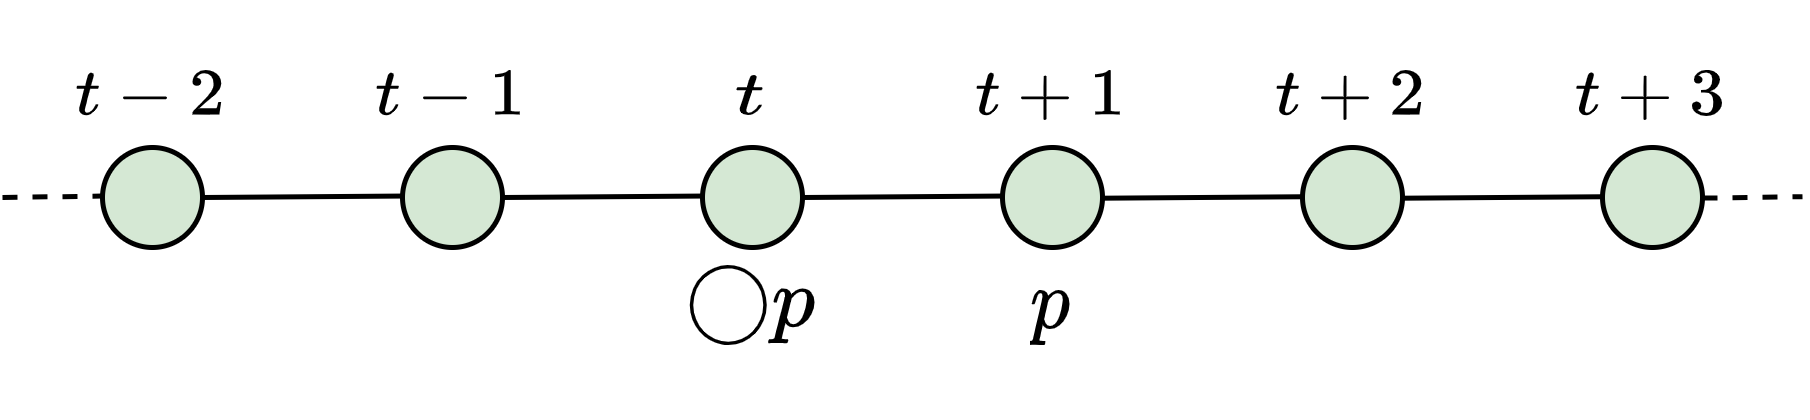
\includegraphics[width=.7\textwidth]{linear_time_logic/images/next_operator.drawio.png}
\end{center}
\begin{examplebox}{All those moments will be lost in time\dots}
    Formalise the following:
    \begin{enumerate}
        \item If you are hungry, next you'll be sad.
        \item If you're hungry and have food, you'll eat next.
        \item Time always increases
    \end{enumerate}
    \tcblower
    \begin{enumerate}
        \item $hungry \Rightarrow \bigcirc sad$
        \item $hungry \land has(food) \Rightarrow \bigcirc (\neg hungry)$
        \item $t = time() \Leftrightarrow \bigcirc (time() = t + 1)$
    \end{enumerate}
\end{examplebox}

\subsection{Always}
\begin{tabular}{c | c r}
    \textcolor{ForestGreen}{TLA+ Supported} & \textcolor{ForestGreen}{LTL Supported} & $\Box p \Leftrightarrow \forall t'. \ (t' \geq t) \Rightarrow p@t'$ \\
\end{tabular}
\begin{center}
    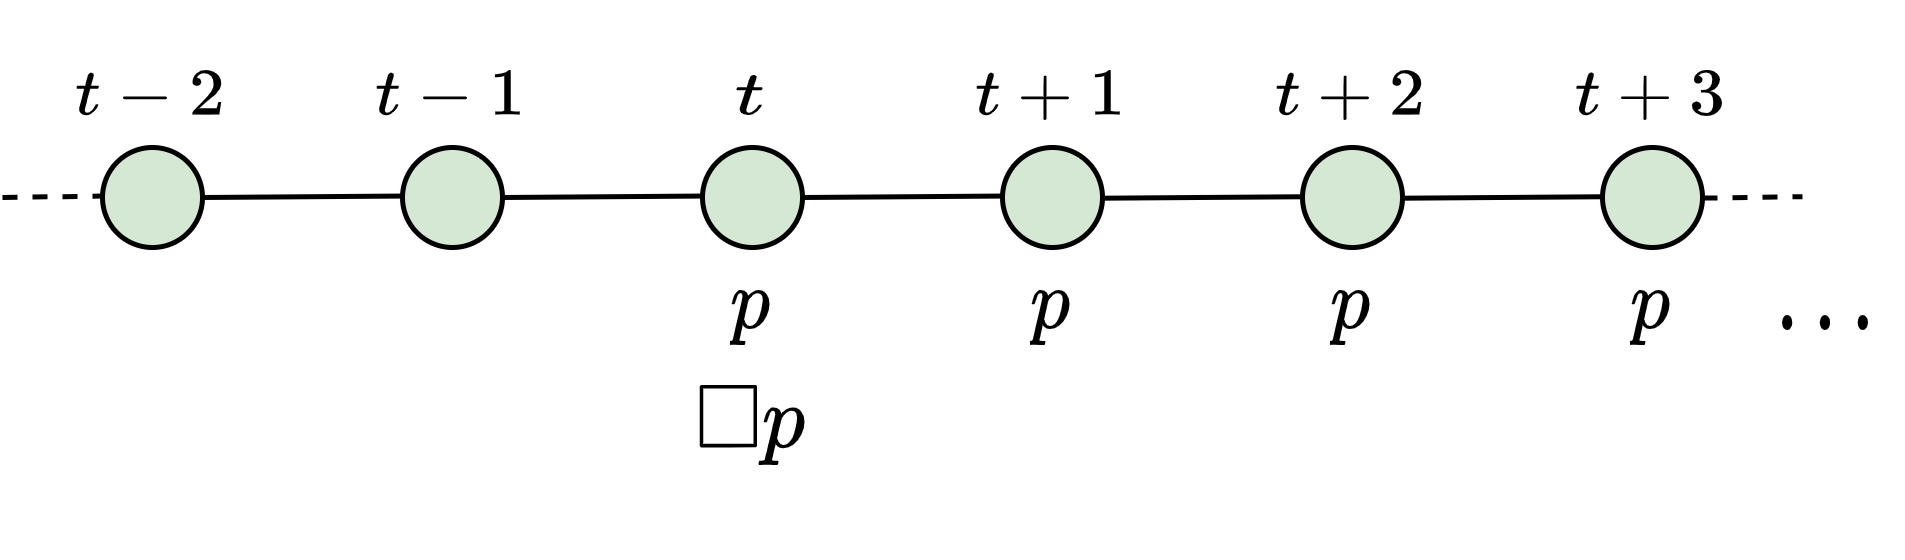
\includegraphics[width=.7\textwidth]{linear_time_logic/images/always_operator.drawio.png}
\end{center}
In TLA+ \textit{ALWAYS} is used to express invariants (true for all states and behaviours).
\begin{examplebox}{There is no next time!}
    Formalise the following:
    \begin{enumerate}
        \item Bad things never happen
        \item If $x = 2$ then it is even
        \item The next counter is always larger than the current
        \item If the config is true, then $x$ always equals $y$
        \item A sequence in which $p$ flips from true to false
    \end{enumerate}
    \tcblower
    \begin{enumerate}
        \item $\Box(\neg bad)$
        \item $\Box(x = 2 \Rightarrow even(x))$
        \item $\Box(counter() = c \Rightarrow \bigcirc (counter() = c + 1))$
        \item $config \Rightarrow \Box(x = y)$
        \item We can formalise as $\Box(p \Leftrightarrow \bigcirc (\neg p))$
    \end{enumerate}
\end{examplebox}

\subsection{Eventually}
\begin{tabular}{c | c r}
    \textcolor{ForestGreen}{TLA+ Supported} & \textcolor{ForestGreen}{LTL Supported} & $\Diamond p \Leftrightarrow \exists t' . \ t' \geq t \land p@t'$ \\
\end{tabular}
\begin{center}
    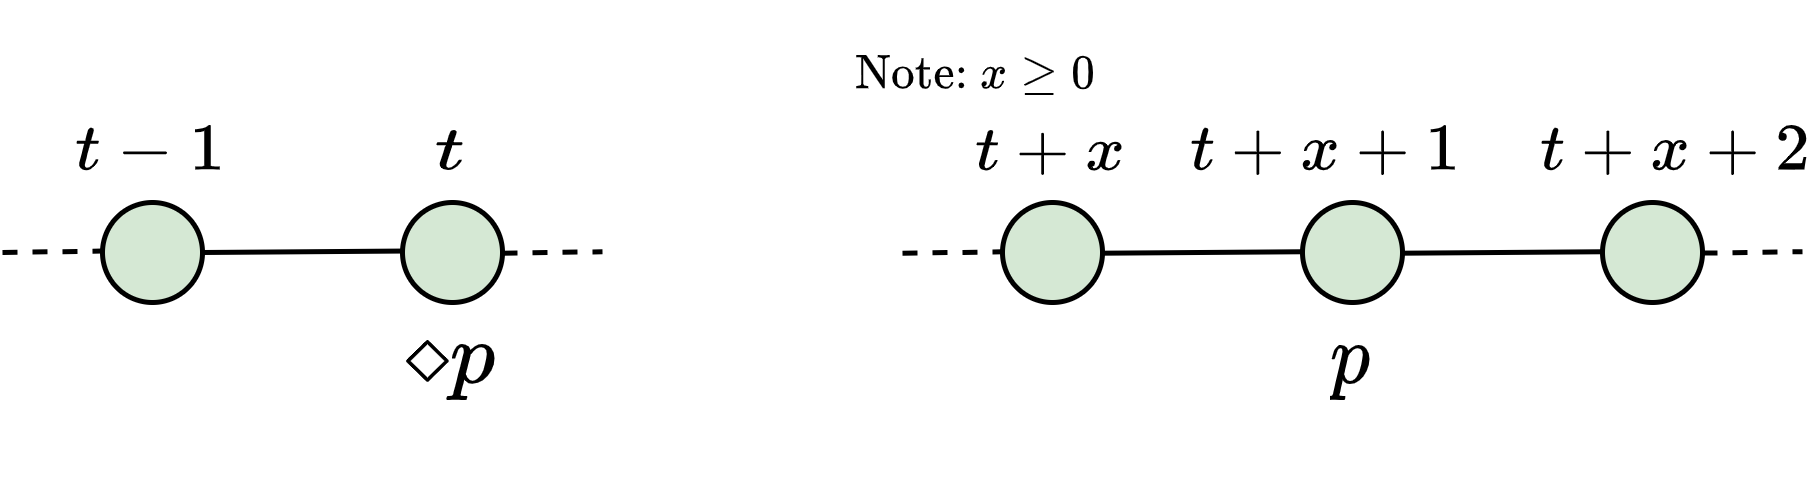
\includegraphics[width=.7\textwidth]{linear_time_logic/images/eventually_operator.drawio.png}
\end{center}
\begin{examplebox}{I'll get around to it!}
    Formalise the following:
    \begin{enumerate}
        \item At one moment $x$ is true, and one moment $y$ is true, but not at the same time.
        \item If $q$ is true and $q$ is false, then $p$ is true next, or some subsequent moment.
        \item Everything sent is eventually delivered.
    \end{enumerate}
    \tcblower
    \begin{enumerate}
        \item $\Diamond x \land \Diamond y \land \Box (\neg (x \land y))$
        \item $q \land \neg p \Rightarrow \bigcirc(\Diamond p)$
        \item $\forall msg . \ \Box(Send(msg) \Rightarrow \Diamond Delivered(msg)) \equiv \forall msg . \ Send(msg) \leadsto Delivered(msg)$
    \end{enumerate}
\end{examplebox}

\subsection{Until}
\begin{tabular}{c | c r}
    \textcolor{red}{Not TLA+} & \textcolor{ForestGreen}{LTL Supported} & $p \ \mathcal{U} \ q \Leftrightarrow \exists t'. \ (t' > t \land q@t' \land (\forall s . \ (t' > s \geq t) \Rightarrow p@s))$ \\
\end{tabular}
\begin{center}
    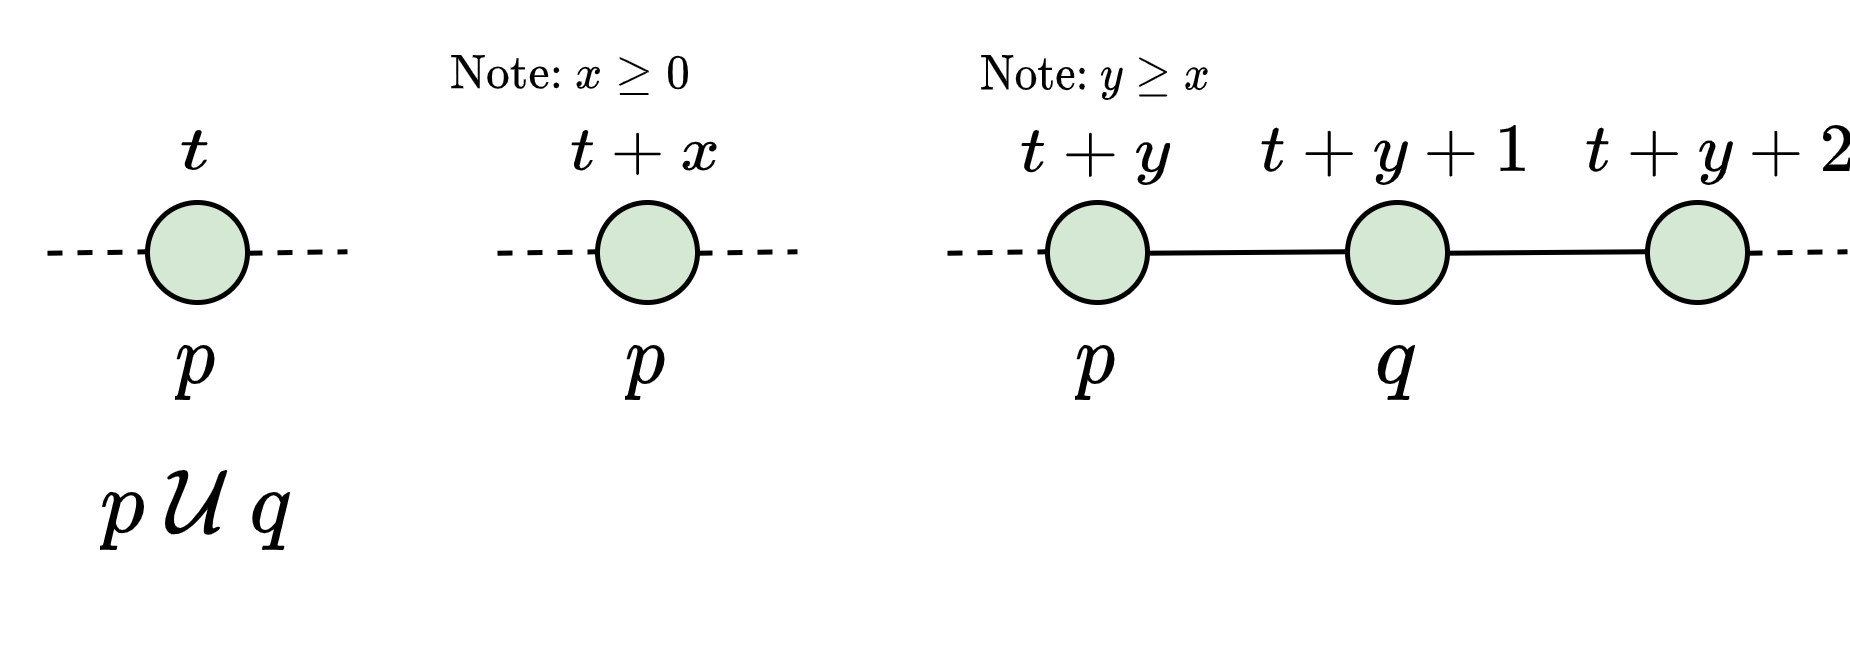
\includegraphics[width=.7\textwidth]{linear_time_logic/images/until_operator.drawio.png}
\end{center}
\begin{itemize}
    \item $p \ \mathcal{U} \ q$ requires that $q$ is eventually true ($\diamond q$), where as \textit{WEAK UNTIL} does not require this.
\end{itemize}
\begin{examplebox}{Gonna live until I die}
    A student attempts to formalise the notion that:
    \\ \centerline{\textit{"Being born always means you are alive until you die"}}
    \\ With the \text{TLT} proposition:
    \[\forall person. \ born(person) \Rightarrow alive(person) \  \mathcal{U} \ die(person)\]
    What issues are there with this answer? Can you suggest a solution?
    \tcblower
    The main issue is that it is possible to:
    \begin{itemize}
        \item Be both alive and dead simultaneously
        \item Come back to life/be born or die multiple times
    \end{itemize}
    We could attempt to fix this by:
    \begin{itemize}
        \item Having the death event prevent any starts to periods of death next \& into the future
        \item Having born occur only once for a person
    \end{itemize}
    \[\forall person . born(person) \Rightarrow (alive(person) \land \neg dead(person)) \ \mathcal{U} \ (\neg alive(person) \land dead(person))\]
\end{examplebox}

\subsection{Always Eventually}
\begin{tabular}{c | c r}
    \textcolor{ForestGreen}{TLA+ Supported} & \textcolor{ForestGreen}{LTL Supported} & $\Box \Diamond p$ \\
\end{tabular}
\begin{center}
    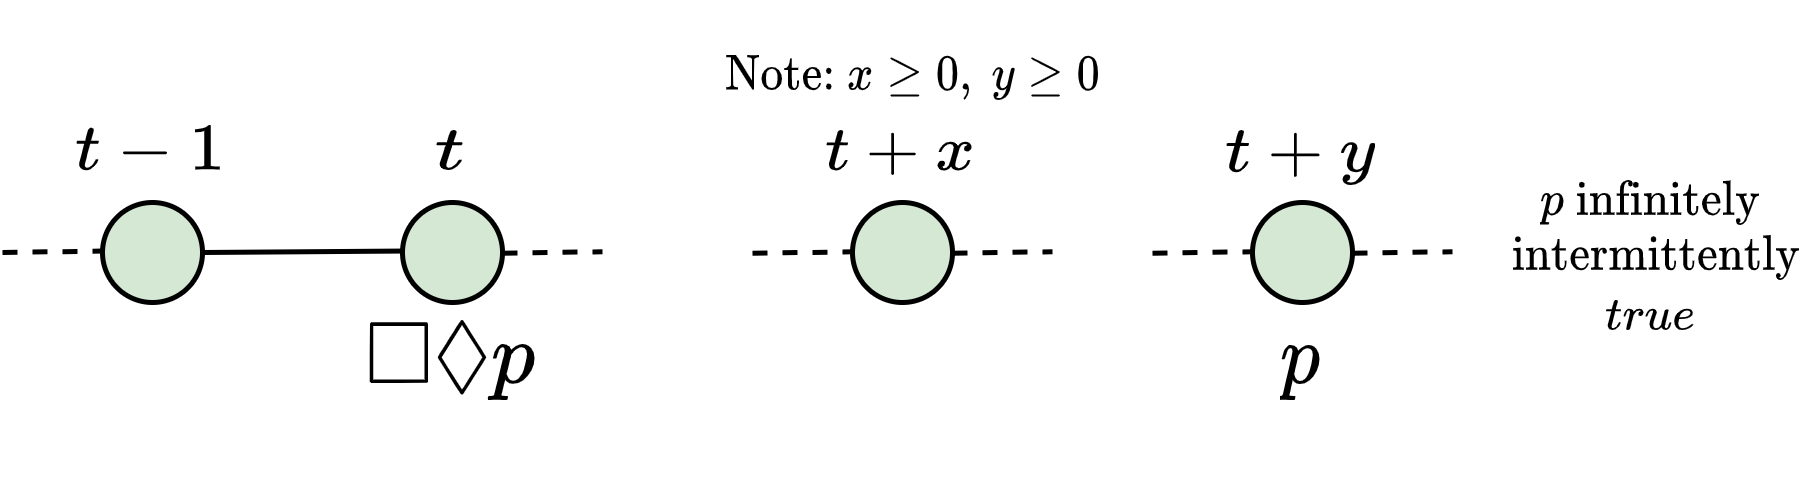
\includegraphics[width=.7\textwidth]{linear_time_logic/images/always_eventually.drawio.png}
\end{center}
$p$ occurs infinitely often, some moments can have $p$ not hold, but there is always another moment in the future where $p$ holds.
\begin{examplebox}{Intermittently True}
    Formalise the following:
    \begin{enumerate}
        \item Sometimes I am hungry
        \item Sometimes I'm hungry
    \end{enumerate}
    \tcblower
    \begin{enumerate}
        \item $\Box \Diamond hungry(me)$
        \item $\Box \Diamond hungry(me) \land \Box (hungry(me) \Leftrightarrow \bigcirc eat(me))$
    \end{enumerate}
\end{examplebox}

\subsection{Eventually Always}
\begin{tabular}{c | c r}
    \textcolor{ForestGreen}{TLA+ Supported} & \textcolor{ForestGreen}{LTL Supported} & $\Diamond \Box p$ \\
\end{tabular}
\begin{center}
    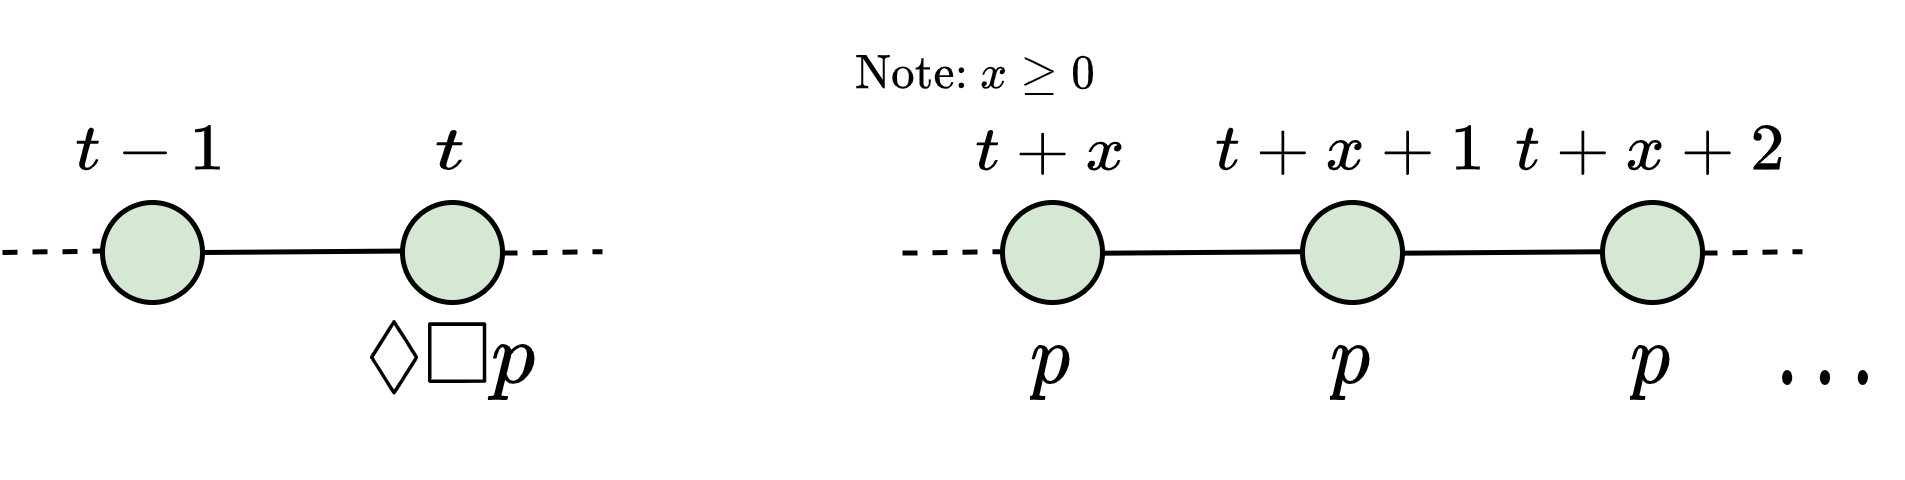
\includegraphics[width=.7\textwidth]{linear_time_logic/images/eventually_always_operator.drawio.png}
\end{center}
\begin{examplebox}{Forever after\dots}
    Model the state of a sticky switch $s$, which will remain stuck to $true$ at some point.
    \tcblower
    \[\Diamond \Box s\]
    Note that a sequence with $s$ going between $true$ and $false$ still satisfies this, it just has to stick to $true$ forever eventually.
\end{examplebox}

\subsection{Equivalences}
\subsubsection{Distribution}
\[
  \begin{matrix}
    \Box (p \land q ) & \equiv & \Box p \land \Box q \\
    \Box (p \lor q ) & \equiv & \Box p \lor \Box q \\
  \end{matrix}
  \qquad \qquad
  \begin{matrix}
    \bigcirc (p \land q) & \equiv & \bigcirc p \land \bigcirc q \\
    \bigcirc (p \lor q) & \equiv & \bigcirc p \lor \bigcirc q \\
  \end{matrix}
  \qquad \qquad
  \begin{matrix}
    (p \land q) \ \mathcal{U} \ r & \equiv & (p \ \mathcal{U} \ r) \land (q \ \mathcal{U} \ r) \\
    p \ \mathcal{U} \ (q \lor r) & \equiv & (p \ \mathcal{U} \ q) \lor (p \ \mathcal{U} \ r) \\
  \end{matrix}
\]

\subsubsection{Dual}
\[
  \begin{matrix}
    \Box \neg p & \equiv & \neg \Diamond p \\
  \end{matrix}
  \qquad \qquad
  \begin{matrix}
    \Diamond \neg p & \equiv & \neg \Box p \\
  \end{matrix}
  \qquad \qquad
  \begin{matrix}
    \bigcirc \neg p & \equiv & \neg \bigcirc p \\
  \end{matrix}
\]
\subsubsection{Miscellanous}
\[
  \begin{matrix}
    \Box \Box p & \equiv & \Box p \\
    \Diamond \Diamond p & \equiv & \Diamond p \\
  \end{matrix}
  \qquad \qquad
  \begin{matrix}
    p \ \mathcal{U} \ (q \ \mathcal{U} \ r) & \equiv & (p \ \mathcal{U} \ q) \ \mathcal{U} \ r & \equiv & p \ \mathcal{U} \ r \\
  \end{matrix}
  \qquad \qquad
  \begin{matrix}
    true \ \mathcal{U} \ p & \equiv & \Diamond p \\
  \end{matrix}
\]

\section{Fairness}
Fairness properties are constraints assumed to be enforced by the system (e.g fairly select which thread to schedule) to ensure the system progresses.
\begin{itemize}
    \item Without fairness constraints the system may fail to make progress (e.g a thread livelocking a system as it waits on an unfair mutex/lock (indefinitely postponed))
    \item Actions can be enabled or disabled. An action is enabled if it can be applied without violating any constraints.
    \item A stuttering step $[A]_v$ which may not change the value of any variables ($[A]_v \triangleq A \lor v = v'$)
    \item A non-stuttering step $\langle A \rangle_v$ must change $v$ ($\langle A \rangle_v \triangleq A \land v \neq v'$).
\end{itemize}
\begin{tcbraster}[raster columns=2,raster equal height]
    \begin{definitionbox}{Strong Fairness}
        \[\Box \Diamond \underline{A} \Rightarrow \Box \Diamond A\]
        If action $A$ is \textit{enabled} infinitely often then it is executed infinitely often.
        \[\textit{Strong Fairness} \Rightarrow \textit{Weak Fairness}\]
        \[SF_v(A) \triangleq \Box \Diamond (\ENABLED \langle A \rangle_v) \Rightarrow \Box \Diamond \langle A \rangle_v\]    
        \begin{minted}{text}
    SF_v(A) == []<>(ENABLED <<A>>_v) 
            => []<><<A>>_V
        \end{minted}
    \end{definitionbox}
    \begin{definitionbox}{Weak Fairness}
        \[\Diamond \Box \underline{A} \Rightarrow \Box \Diamond A\]
        If action $A$ is eventually permanently \textit{enabled}, then it is executed infinitely often.
        \[\]
        \[WF_v(A) \triangleq \Diamond \Box (\ENABLED \langle A \rangle_v) \Rightarrow \Box \Diamond \langle A \rangle_v\]
        \begin{minted}{text}
    WF_v(A) == <>[](ENABLED <<A>>_v) 
            => []<><<A>>_v
        \end{minted}
    \end{definitionbox}
\end{tcbraster}
\begin{definitionbox}{Absolute Fairness}
    \[\Box\Diamond A \qquad \qquad \textit{Absolute Fairness} \Rightarrow \textit{Strong Fairness}\]
    Action A is executed infinitely often, even if it is not enabled.
\end{definitionbox}

\section{Safety}
We can assert safety properties in each step.
\begin{examplebox}{Safety Property}
    Explain the safety properties of the following TLA+ spec.
    \begin{center}
        \begin{minipage}{.49\textwidth}
            \[Spec \triangleq Init \land \Box [Next]_{Vars}\]
        \end{minipage} \hfill \begin{minipage}{.49\textwidth}
            \begin{minted}{text}
Spec == Init /\ [][Next]_Vars
            \end{minted}
        \end{minipage}    
    \end{center}
    \tcblower
    If $Init$ is not true, or there is some state for which $Next$ is false, but some $Vars$ change, then there is a safety property violation.
\end{examplebox}
\begin{examplebox}{Deadlocked}
    Explain the safety properties of the following TLA+ spec.
    \begin{center}
        \begin{minipage}{.49\textwidth}
            \[NoDeadlock \triangleq \Box(\ENABLED Next)\]
        \end{minipage} \hfill \begin{minipage}{.49\textwidth}
            \begin{minted}{text}
NoDeadlock == [](ENABLED Next)
            \end{minted}
        \end{minipage}    
    \end{center}
    \tcblower
    Safety property asserting that there is no state for which Next is disabled/cannot be satisfied.
\end{examplebox}

\section{Liveness}
Properties asserting what must happen eventually. As they cannot be violated in finite steps, we must consider infinite behaviours through temporal logic.
\begin{itemize}
    \item Typically in TLA+ rather than an ad-hoc/specific implementation per spec, we use some conjunction of $WF_v(A)$ and $SF_v(A)$ are used to specify the liveness properties to be checked.
\end{itemize}
\begin{minipage}{.49\textwidth}
    \[\begin{split}
        Fairness & \triangleq WF_v(Action1) \land SF_v(Action2) \land \dots \\
        Spec & \triangleq Init \land \Box[Next]_{Vars} \land Fairness \\
        LivenessProp & \triangleq \dots \ (\text{Some temporal formula}) \\
    \end{split}\]
\end{minipage} \hfill \begin{minipage}{.49\textwidth}
    \begin{minted}{text}
    Fairness == WF_v(Action1) /\ SF_v(Action2) /\ ...
        Spec == Init /\ [][Next]_Vars /\ Fairness
LivenessProp == \* Some temporal formula
    \end{minted}
\end{minipage}

\subsection{LiveClock12}
We first develop a basic 12 hour clock.
\\ \begin{minipage}{.35\textwidth}
    \tlatex
\@x{}\moduleLeftDash\@xx{ {\MODULE} Clock12}\moduleRightDash\@xx{}%
\@x{ {\EXTENDS} Naturals}%
\@x{ {\VARIABLE} hour}%
\@pvspace{8.0pt}%
\@x{}%
\@y{\@s{0}%
 12 hour clock state constraint
}%
\@xx{}%
\@x{ Type \.{\defeq} hour \.{\in} 1 \.{\dotdot} 12}%
\@x{}\midbar\@xx{}%
\@x{}%
\@y{\@s{0}%
 Initial and \ensuremath{Next} Action
}%
\@xx{}%
\@x{ Init\@s{4.12} \.{\defeq} Type}%
\@x{ Next \.{\defeq} hour \.{'} \.{=} ( hour \.{\%} 12 ) \.{+} 1}%
\@pvspace{8.0pt}%
\@x{ Spec\@s{1.46} \.{\defeq} Init \.{\land} {\Box} [ Next ]_{ hour}}%
\@x{}\midbar\@xx{}%
\@pvspace{8.0pt}%
\@x{ Typed \.{\defeq} {\Box} Type}%
\@x{}\bottombar\@xx{}%

\end{minipage} \hfill \begin{minipage}{.32\textwidth}
\inputminted{text}{linear_time_logic/code/Clock12.tla}
\end{minipage} \hfill \begin{minipage}{.22\textwidth}
\inputminted{text}{linear_time_logic/code/Clock12.cfg}
\end{minipage}
\vspace{.3cm}
\\ We can then extend this module with fairness and liveness properties.
\vspace{.3cm}
\\ \begin{minipage}{.48\textwidth}
    \tlatex
\@x{}\moduleLeftDash\@xx{ {\MODULE} LiveClock12}\moduleRightDash\@xx{}%
\@x{ {\EXTENDS} Clock12}%
\@pvspace{8.0pt}%
\@x{}%
\@y{}%
\@xx{}%
\@x{ Fairness\@s{0.63} \.{\defeq} {\WF}_{ hour} ( Next )}%
\@x{ LiveSpec \.{\defeq} Spec \.{\land} Fairness}%
\@x{}\midbar\@xx{}%
\@x{}%
\@y{\@s{0}%
 There is always another hour
}%
\@xx{}%
 \@x{ AlwaysTick \.{\defeq} {\Box} {\Diamond} {\langle} Next {\rangle}_{
 hour}}%
\@pvspace{8.0pt}%
\@x{}%
\@y{\@s{0}%
 All hour states are always used in the future
}%
\@xx{}%
 \@x{ AllTimes \.{\defeq} \A\, hr \.{\in} 1 \.{\dotdot} 12 \.{:} {\Box}
 {\Diamond} ( hour \.{=} hr )}%
\@x{}\bottombar\@xx{}%

\end{minipage} \hfill \begin{minipage}{.48\textwidth}
\inputminted{text}{linear_time_logic/code/LiveClock12.tla}
\end{minipage}
\vspace{.3cm}
\inputminted{text}{linear_time_logic/code/LiveClock12.cfg} 
\subsection{Alternating Bit Protocol}
\begin{center}
    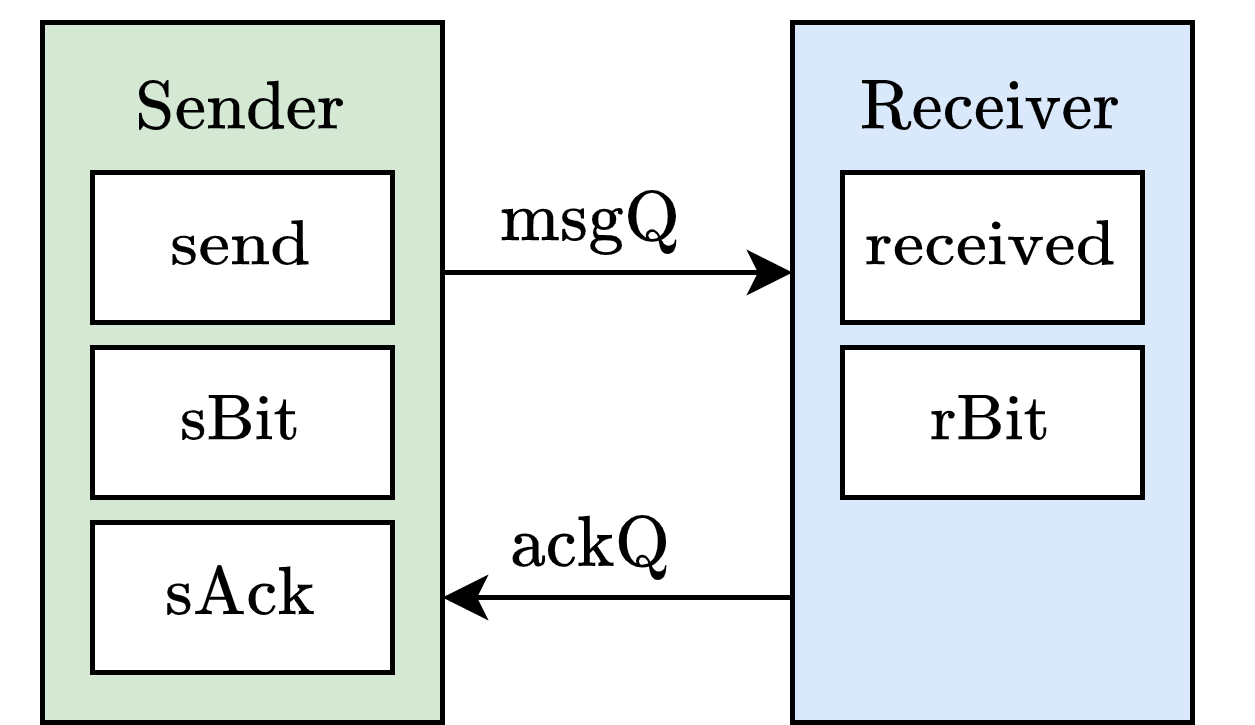
\includegraphics[width=.4\textwidth]{linear_time_logic/images/alt_bit_protocol.drawio.png}
\end{center}
\unfinished
% \subsubsection{TLA+}
% \* Abstract Module
% \subsubsection{Code}
% \inputminted{text}{linear_time_logic/code/AltBit.tla}
% \subsubsection{Configuration}
% \inputminted{text}{linear_time_logic/code/AltBit.cfg}